\documentclass[man, floatsintext]{apa6}
% floatsintext so that figures show up where we want them to (https://www.tug.org/pracjourn/2012-1/beitzel/beitzel.pdf) 
\usepackage{lipsum}
\usepackage{amsmath}

\usepackage[american]{babel}
\usepackage{ulem}
\usepackage{graphicx} 
\usepackage{csquotes}
\usepackage{hyperref}
\usepackage[style=apa,sortcites=true,sorting=nyt,backend=biber]{biblatex}
\DeclareLanguageMapping{american}{american-apa}
\addbibresource{project1.bib}

\title{Analysis of Customer Churn at Telco}

\shorttitle{Customer Churn}

\author{Pedro Uria, Sean Pili, and Zachary Buckley}

\affiliation{George Washington University}

\abstract{
  TODO: This is the abstract.
}

\begin{document}
\maketitle

\section{Introduction and Background Research}
\paragraph{Churn Rate}

In business, churn rate is the percentage of a company's customers that terminate their relationship with that company \textbf{during a given time period}. In the telecommunications industry, churn rates can be especially high because there is fierce competition and the market is saturated. In fact, in their (\textbf{who is they}?) study of factors that explain customer churn rates for an Indian telecommunications company Asamoah et. al, \textbf{they} mention that ``worldwide, the rate of customer churn in the telecom service industry ranges from 20 percent to 40 percent per year'' (224) \textbf{I guess you want to insert a reference here?}. If a company loses 20-40 percent of its existing customer base every year, that can have a significant \textbf{and} negative \sout{on} effect on its revenue, regardless \textbf{of} how many new customers they obtain.  Consequently, many companies in saturated markets keep track of monthly, quarterly or yearly churn rates in an attempt to identify defining characteristics of customers who churn, in order to predict and eventually reduce their customer churn rate. 

Much of the scientific research on reducing customer churn across all industry verticals involves using logistic regression or \textbf{other} classification methods to predict which customers will churn in a given \textbf{time} period (typically monthly.) Common features used \sout{to classify which customers will churn across different industry verticals} \textbf{as classifiers} include different aspects of customer purchasing behavior, their tenure (the length of a customer's relationship with a company), their account charges,  and frequency of their transactions (depending on the type of business). In 2015 Jarvis et al. ran an analysis on consumer data from an Australian streaming DVD rental service to determine if adding features that measure ``customer satisfaction, attitude and commitment'' to models meant to classify whether or not a customer will churn would increase their prediction accuracy.  Interestingly, Jarvis et. al. found that ``the most significant predictor of churn in [customer purchasing habits, satisfaction and attitude] was a measure of uncertainty and commitment: the number of times a customer changed their subscription plan''. Jarvis et. al did not explain how the customers changed their plans, (i.e. did the customers add or subtract services from their plans or alter other aspects of their plans entirely?)  Additionally

\hspace{0.5mm}

\paragraph{Telco Dataset}

The Telco Customer Churn Dataset we will be using throughout this paper contains information about the customers from an unidentified telecommunications company. The data was uploaded to \href{https://www.kaggle.com/blastchar/telco-customer-churn}{Kaggle} by a user named blastchar. \cite{blastchar_2018} ??? The dataset originates from a sample dataset provided by IBM for exploring the capabilities of IBM's Watson Analytics services. IBM uses the data in a walkthrough of building a model for predicting whether a customer will leave the company, with the explicit goal of creating better customer retention programs. \cite{ibm_telco_2015} \textbf{For this to work we need to create a bibliography}. There are a number of sample data sets provided by IBM for similar walkthroughs related to their Watson Analytics system. \cite{ibm_data_2015} We were unable to determine conclusively if the Telco Dataset we're interested in for this paper was based on data from a real telecommunications company, or if the data was synthetically generated for the purposes of demonstrating the Watson Analytics system's capabilities.

\hspace{0.5mm}

\section{Research Question, Hypotheses and Methods (variable explanations)}
\paragraph{Research Question}

Are there significant relationships with the following variables and Churn:
\begin{itemize}
\item{Contract Type}
\item{Paperless Billing}
\item{Partner}
\item{Device Protection}
\item{Tech Support}
\item{Online Backup}
\end{itemize}

Original Research Question:
Is Churn rate independent of the type of contract a customer holds and if the average tenure of customers who churned is different that the average tenure of customers who are remaining with the company.

\paragraph{Hypothesis}

D

\paragraph{Methods}

E

\section{Overview of the findings including EDA and model results}

\paragraph{Contract Type}

C

\paragraph{Billing}

In this section we first did \textit{EDA} on \texttt{MonthlyCharges}, a continuous variable that gives the amount of dollars charged to a customer each month (thus, in this case we shall not use a $\chi^2$-test, which only makes sense for categorical data). The goal was to have a first look at how this variable behaved for customers who churned and for customers who did not churn, in order to asses which statistical test to use to check our alternate hypothesis. 

\hspace{0.5mm}

\noindent\begin{minipage}{0.54\textwidth}
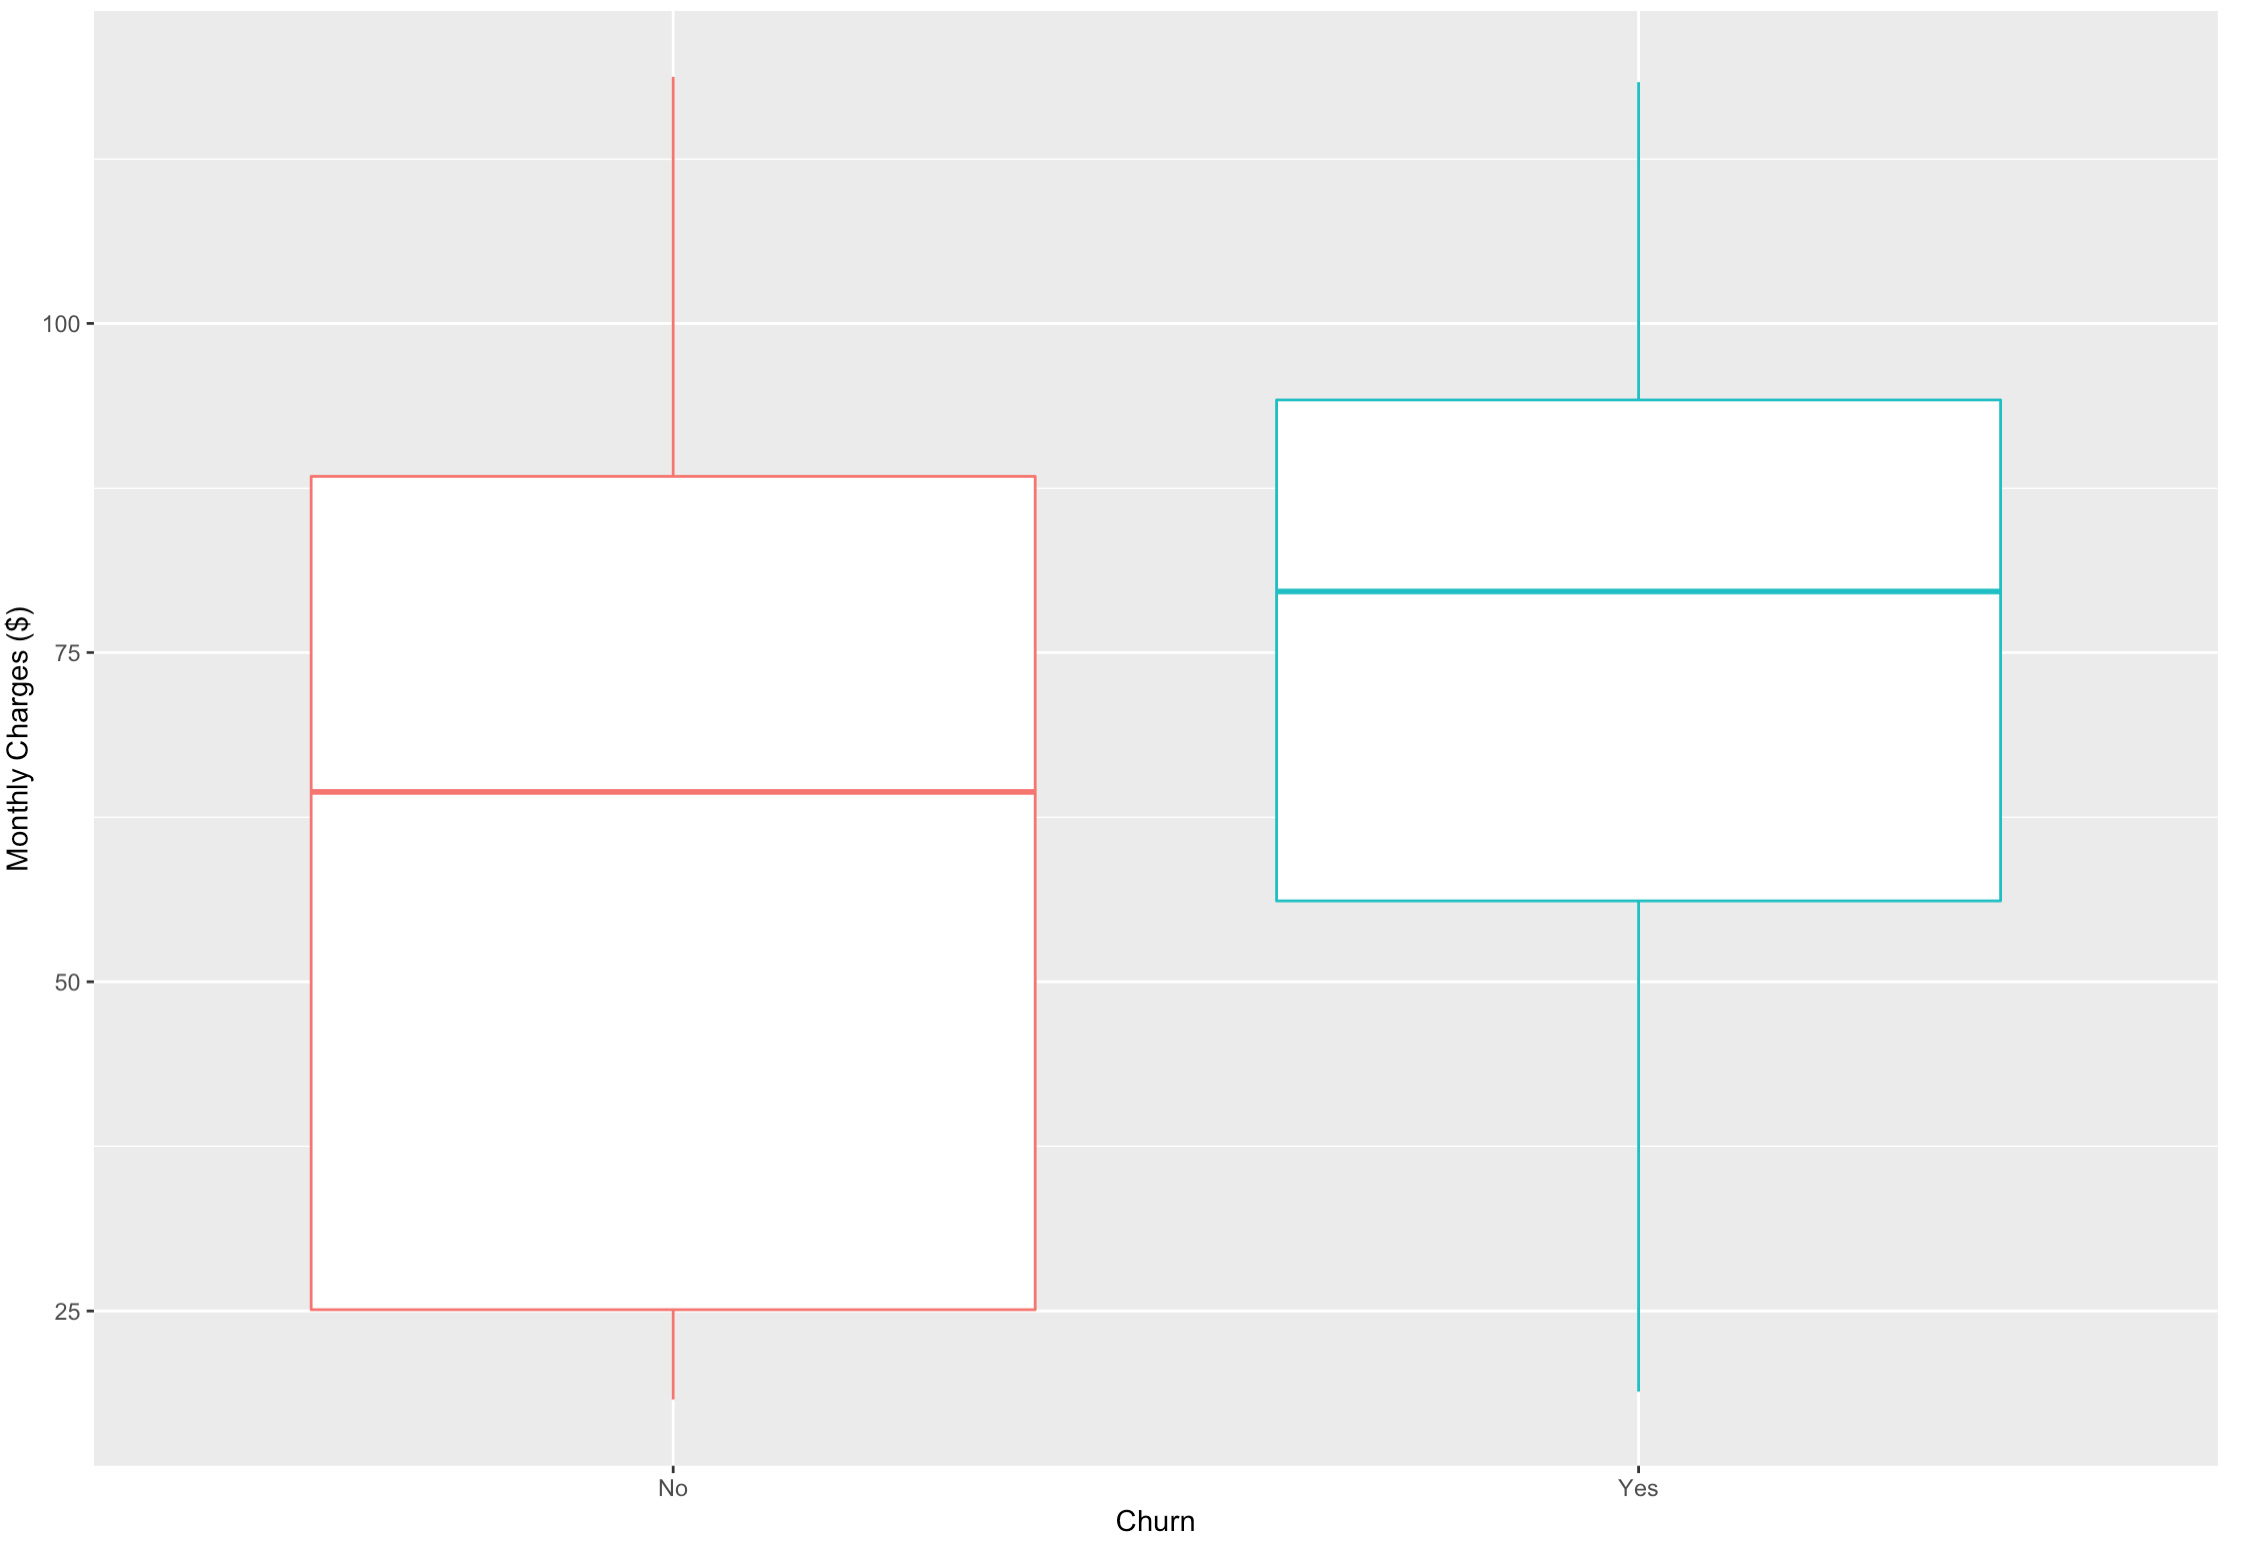
\includegraphics[width = \linewidth]{boxplot_MonthlyChargesvsChurn}
\end{minipage}
\hfill
\begin{minipage}{0.45\textwidth} On the left there is a boxplot for \texttt{MonthlyCharges}, grouped by \texttt{Churn}. We can see how the variances are clearly different, and because of this we can't use a Student's $t$-test to tell whether $\overline{X}_{\text{Churn}} = \overline{X}_{\text{NotChurn}}$ or not. Instead, we will use a Welch's $t$-test, which does not assume equality of variances.
 
\end{minipage}
\noindent\begin{minipage}{0.5\textwidth}
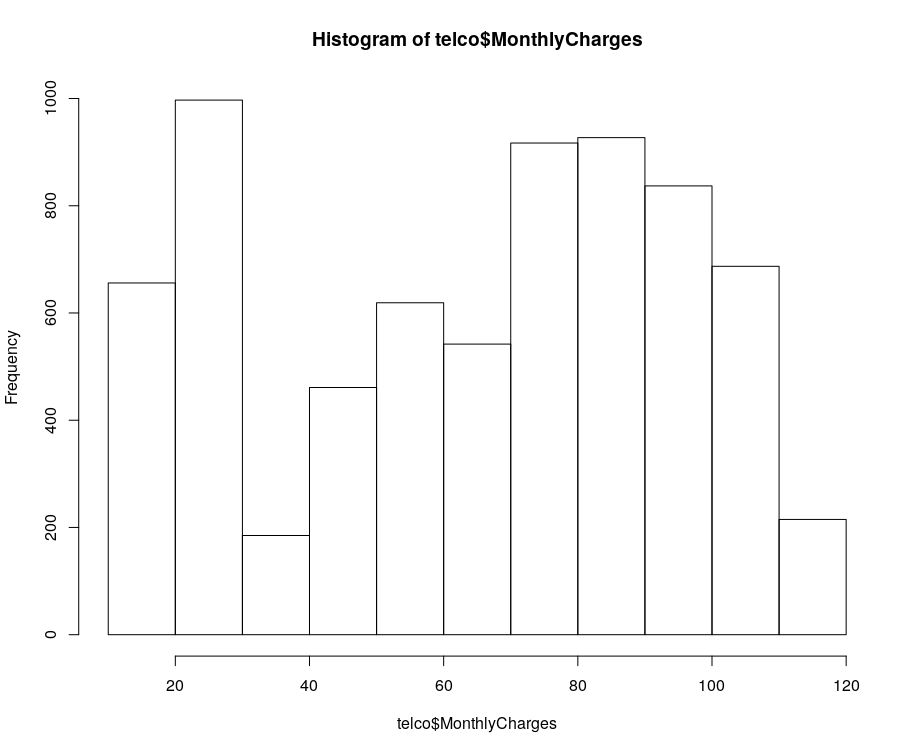
\includegraphics[width = \linewidth]{hist_MonthlyCharges}
\end{minipage}
\hfill
\begin{minipage}{0.45\textwidth} Notice how the distribution of the monthly charges is not normally shaped. However, what we are comparing are means, and the Central Limit Theorem assures us that these means will follow a normal distribution for a large enough sample size (our case), which enables us to perform the Welch's $t$-test. 
\end{minipage}

\hspace{0.5mm}

Upon running this test on R, we get a $p$-value $< 2.2 \cdot 10^{-16}$, so we reject $H_0$ and say that the two means are statistically different at the $\alpha = 0.05$ level of significance. In particular, it seems that customers who churned are paying more on average that customers who have not churned.

\hspace{0.5mm}

\paragraph{Tenure}

The process for \texttt{Tenure} was analogous to the one for \texttt{MonthlyCharges}, as this continuous variable presented similar differences in variance and is also non-normally shaped. 

\hspace{0.5mm}

\noindent\begin{minipage}{0.485\textwidth}
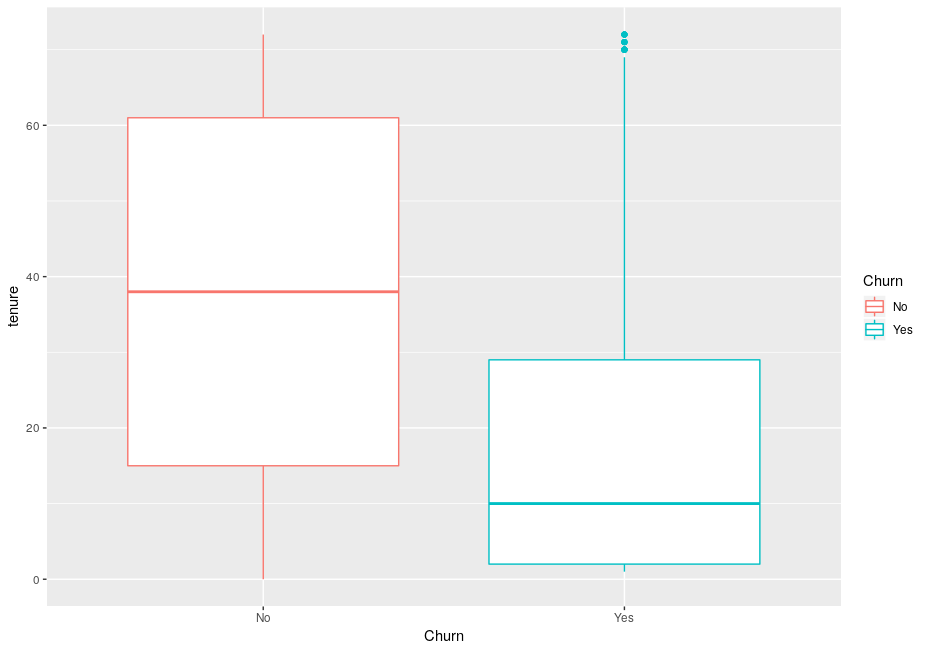
\includegraphics[width = \linewidth]{boxplot_tenurebyChurn}
\end{minipage}
\hfill
\begin{minipage}{0.5\textwidth} 
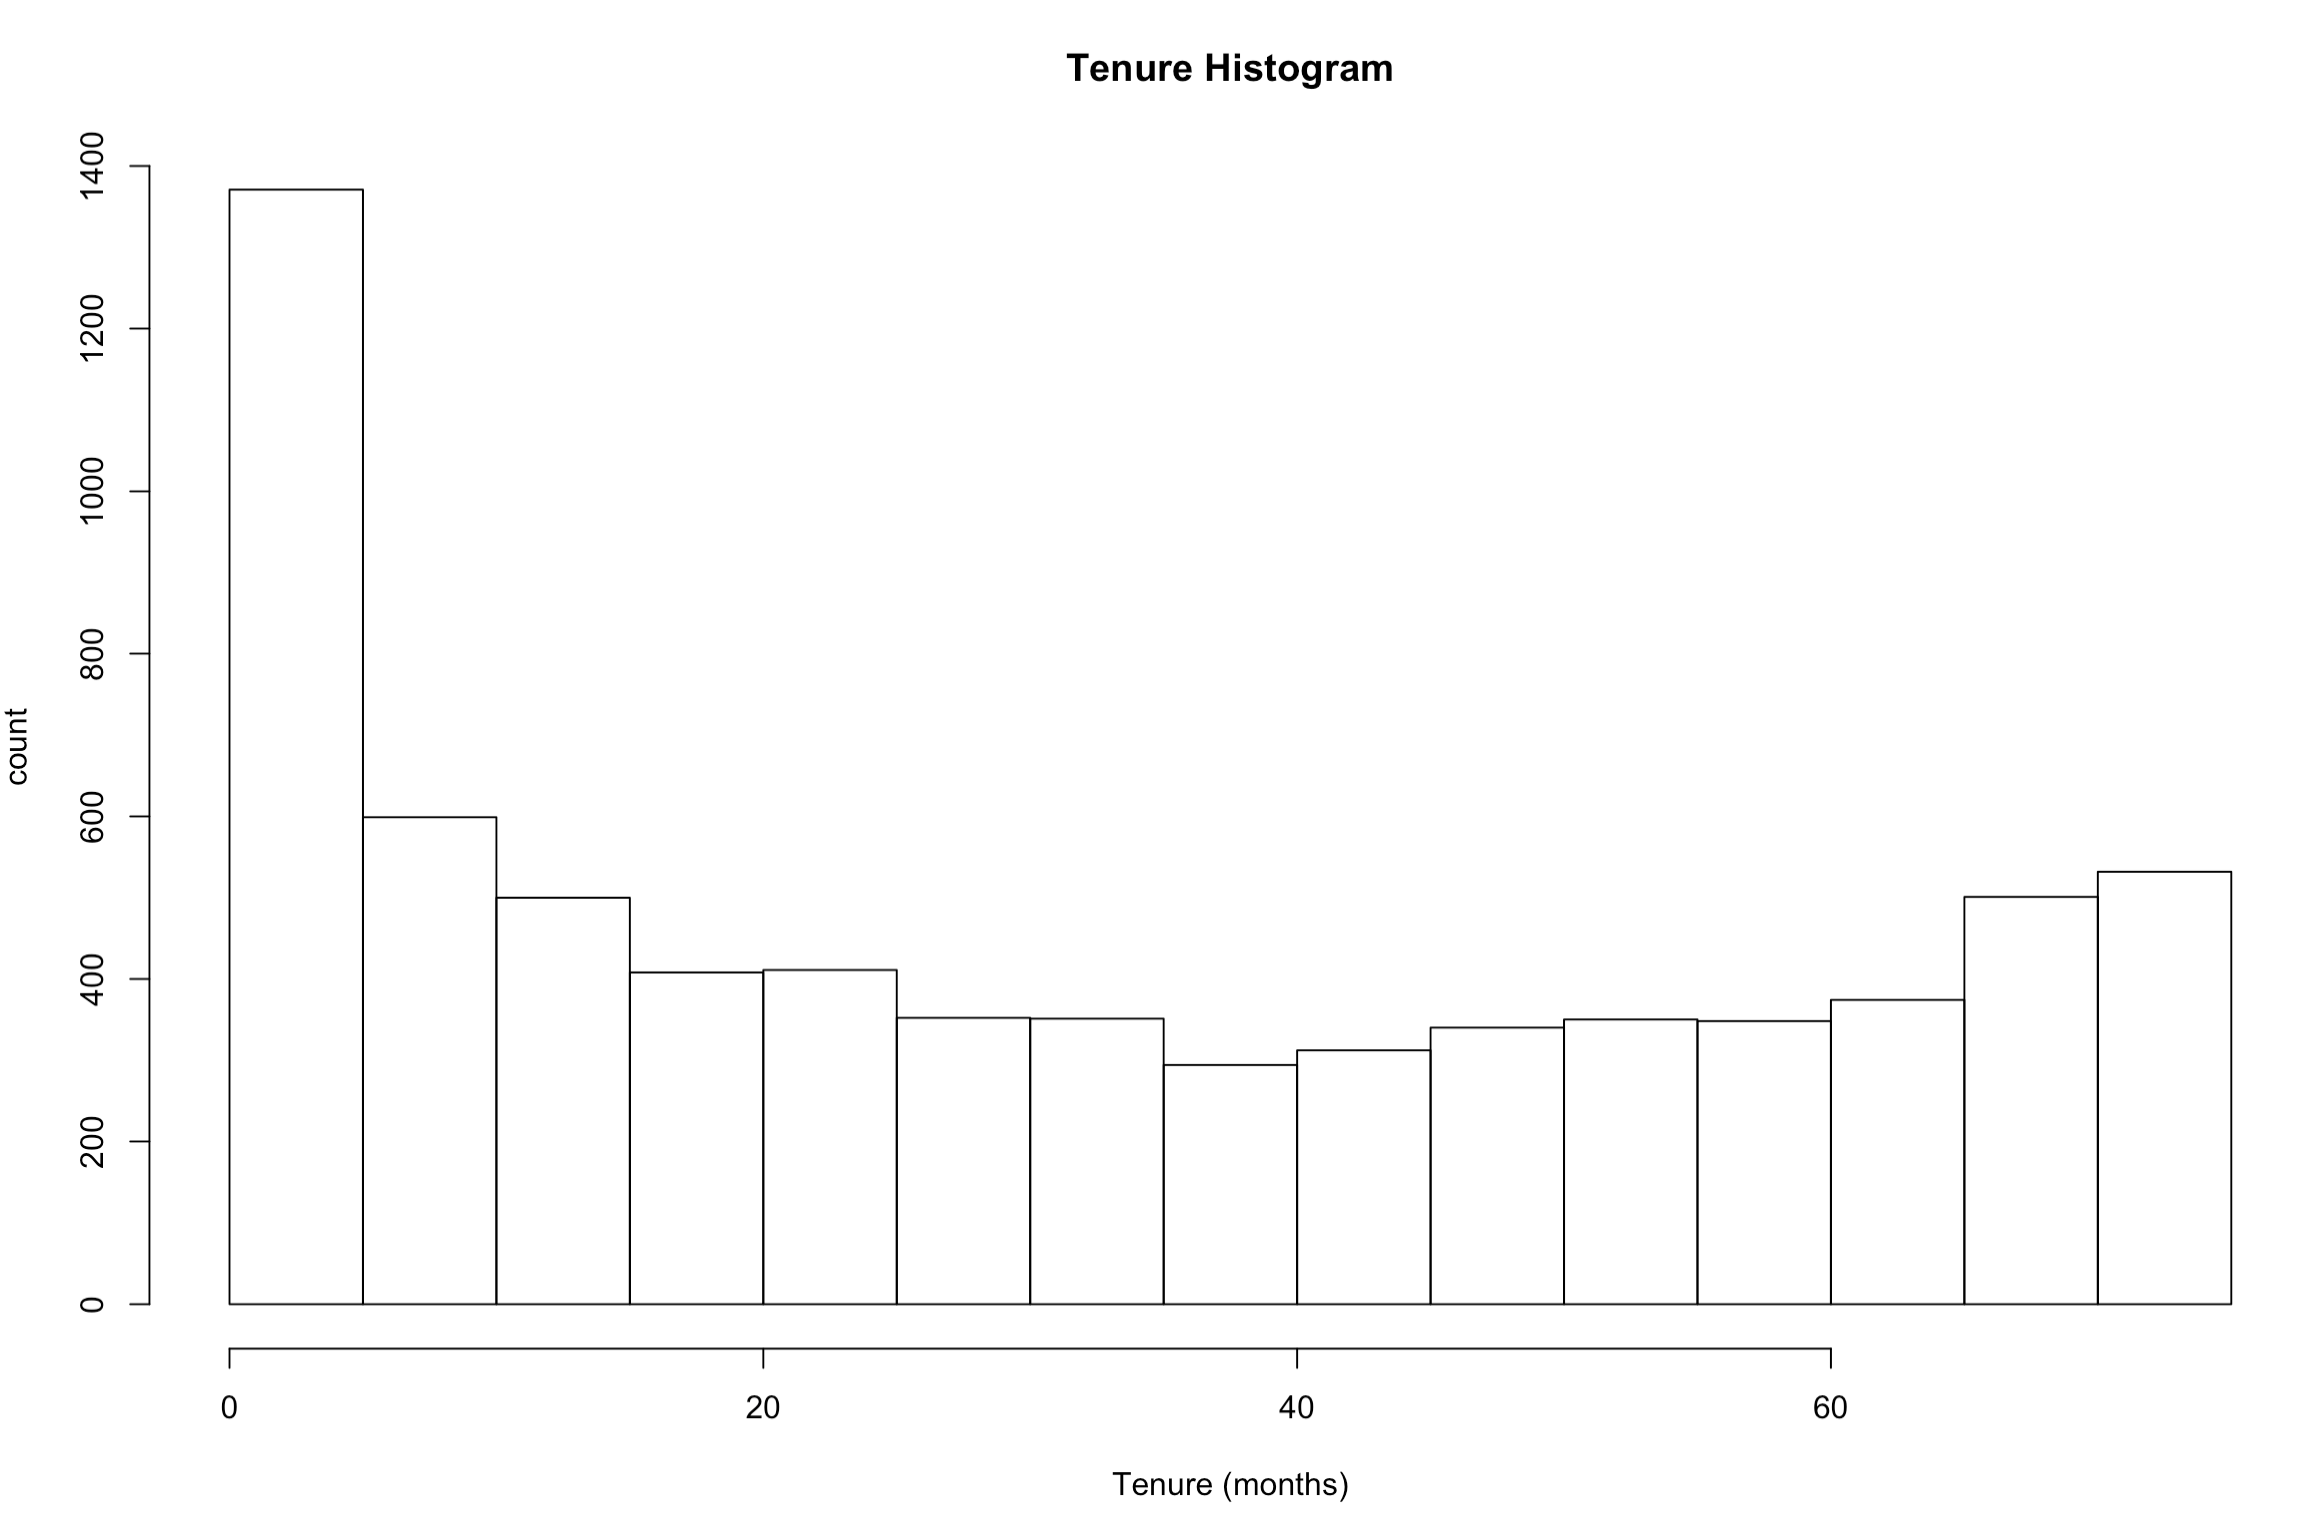
\includegraphics[width = \linewidth]{histogram_Tenure}
\end{minipage}

\hspace{0.5mm}

In this case, we also get a very small $p$-value (again $< 2.2 \cdot 10^{-16}$), so we reject the null hypothesis that  $\overline{X}_{\text{Churn}} - \overline{X}_{\text{NotChurn}} = 0$ and say that at the $5 \%$ significance level, $\overline{X}_{\text{Churn}} \neq \overline{X}_{\text{NotChurn}}$. Customers who haven't churned have been longer on average with the company. 


\section{A discussion of what conclusions can be drawn as a result of your project.}
G
\appendix
\section{Best Variables for Linear Regression?}
\newpage
\printbibliography
\end{document}
